\documentclass[aspectratio=1610]{beamer}

\usetheme{unnslides}
\usefonttheme{professionalfonts}

\usepackage[T2A]{fontenc}
\usepackage[utf8]{inputenc}
\inputencoding{utf8}
\usepackage{listings}
\usepackage{graphicx}
\usepackage{caption}
\usepackage{cmbright}
\usepackage{fontspec}
\usepackage{unicode-math}
\usepackage{amsfonts}
\usepackage{subfig}
\usepackage{tikz}

\captionsetup[subfigure]{labelformat=empty}
\captionsetup[figure]{labelformat=empty}

\setmainfont{CMU Sans Serif}
\setromanfont{CMU Sans Serif}
\setsansfont{CMU Sans Serif}

\setlength{\tabcolsep}{1pt}

\usepackage{polyglossia}
\setmainlanguage{russian}
%\setbeamertemplate{itemize item}{\color{black}$\blacktriangleright$}

\DeclareMathOperator*{\argmax}{arg\,max}
\DeclareMathOperator*{\argmin}{arg\,min}
\DeclareMathOperator{\sign}{sign}
\DeclareMathOperator{\re}{Re}

\graphicspath{ {../images/}{img/} }

%set pages numeration
\newcommand\numbered{\setbeamertemplate{footline}{%
  \vspace{-10em}
   \raisebox{5pt}{\makebox[\paperwidth]{%
     \hfill\makebox[10pt]{%
       \usebeamerfont{footline}\usebeamercolor[fg]{footline}
       \insertframenumber}}}}}
\newcommand\unnumbered{\setbeamertemplate{footline}{}}

\title{Разработка и исследование способов распределения ресурсов в
параллельных алгоритмах глобальной оптимизации}
\author{\textbf{Соврасов~В.В}, научный руководитель: Баркалов~К.А.}
\institute{ННГУ им. Н.И.~Лобачевского}
\date{}

\begin{document}
\numbered
{
\unnumbered
\begin{frame}[noframenumbering,plain]
\titlepage
\end{frame}
}

\begin{frame}
  \frametitle{Структура работы}
  \begin{enumerate}
    \setlength{\itemindent}{.1in}
    \item[Глава 1.] Методы редукции размерности, их сравнение
    \item[Глава 2.] Сравнение актуальных методов глобальной оптимизации
    \item[Глава 3.] Метод для решения множества задач с ограничениями
  \end{enumerate}
\end{frame}


\begin{frame}
  \frametitle{Постановка задачи глобальной оптимизации}
  \begin{columns}
    \begin{column}{0.5\textwidth}
      \begin{displaymath}
        \begin{array}{cr}\\
          \varphi(y^*)=\min\{\varphi(y):y\in G\},\:G=D \cap \{y:\\
           g_j(y)\leqslant 0, 1\leqslant j\leqslant m\},
        \end{array}
      \end{displaymath}
      где \(D\) -- прямоугольник в \(\mathbb{R}^N\),
      \(\varphi(y),\:g_j(y)\) -- многоэкстремальные функции, удовлетворяющие условию Липшица в \(D\):
      \begin{displaymath}
          |f(y_1)-f(y_2)|\leqslant L\Vert y_1-y_2\Vert,y_1,y_2\in D,
      \end{displaymath}
      где \(L>0\) -- константа Липшица, а \(||\cdot||\) обозначает \(l_2\)-норму в \(\mathbb{R}^N\).
    \end{column}
    \begin{column}{0.5\textwidth}
      \centerline{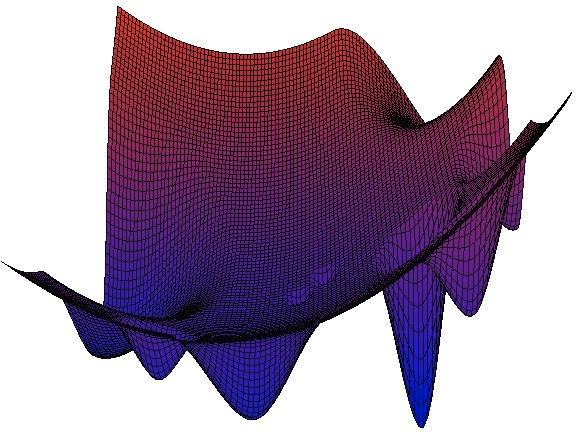
\includegraphics[width=0.9\textwidth]{img/gkls.png}}
    \end{column}
  \end{columns}
\end{frame}

\begin{frame}
  \frametitle{Постановка задачи глобальной оптимизации}
  Рассмотрим множество из \(q\) глобальной оптимизации с ограничениями-неравенствами:
  \begin{equation}
    \label{eq:many_problems}
    \min\left\{\varphi_1(y), y\in G_1 \right\}, \min\left\{\varphi_2(y), y\in G_2\right\},...,
  \min\left\{\varphi_q(y), y\in G_q\right\}.
  \end{equation}
  Будем считать, что метод оптимально распоряжается ресурсами, если при его остановке на некоторой итерации
  решение всех задач получено с одинаковой точностью. Такого свойства можно добиться, потребовав
  от метода равномерной сходимости на всём множестве задач:
  \begin{equation}
    \exists \varepsilon > 0: \forall s>1, \forall i,j\in\{1,\dots,q\}\;
      \frac{\Vert \overline{y_i}^*(s) - y_i^*\Vert_\infty}{\Vert \overline{y_j}^*(s) - y_j^*\Vert_	\infty} \leqslant \varepsilon,
  \end{equation}
  где \(s\) это количество итераций метода оптимизации, \(\tilde{y_i}(s)^*\) это приближение к решению, полученное методом в задаче \(i\)
  из множества (\ref{eq:many_problems}) на итерации \(s\).

\end{frame}

\begin{frame}
  \frametitle{Решение множества задач}
  Упомянутые множества задач могут возникнуть, например, в следующих случаях:
  \begin{itemize}
    \item наличие у непрерывной задачи дискретного параметра, который принимает ограниченный диапазон значений;
    \item набор задач получен при скаляризации задачи многокритериальной оптимизации.
  \end{itemize}
\textbf{Возможные подходы}:
  \begin{itemize}
    \item решать каждую задачу независимо;
    \item разработать метод оптимизации, решающий все задачи "одновременно", в каждый момент времени приоритизируя одну из них.
  \end{itemize}
\end{frame}

\begin{frame}
  \frametitle{Редукция размерности с помощью развёрток}
  \begin{center}
  Кривая типа Пеано \(y(x)\) позволяет снизить размерность исходной задачи оптимизации:
  \begin{gather}
    D_e=\lbrace y\in \mathbb{R}^N:-2^{-1}\leqslant y_i\leqslant 2^{-1},1\leqslant i\leqslant N\rbrace=\{y(x):0\leqslant x\leqslant 1\} \nonumber \\
    \min\{\varphi(y): y\in D\}=\min\{\varphi(y(x)): x\in [0,1]\} \nonumber
  \end{gather}
  \(y(x)\) является негладкой непрерывной функцией, отображающей отрезок \([0,1]\) на гиперкуб \(D_e\).
  \begin{figure}[ht]
    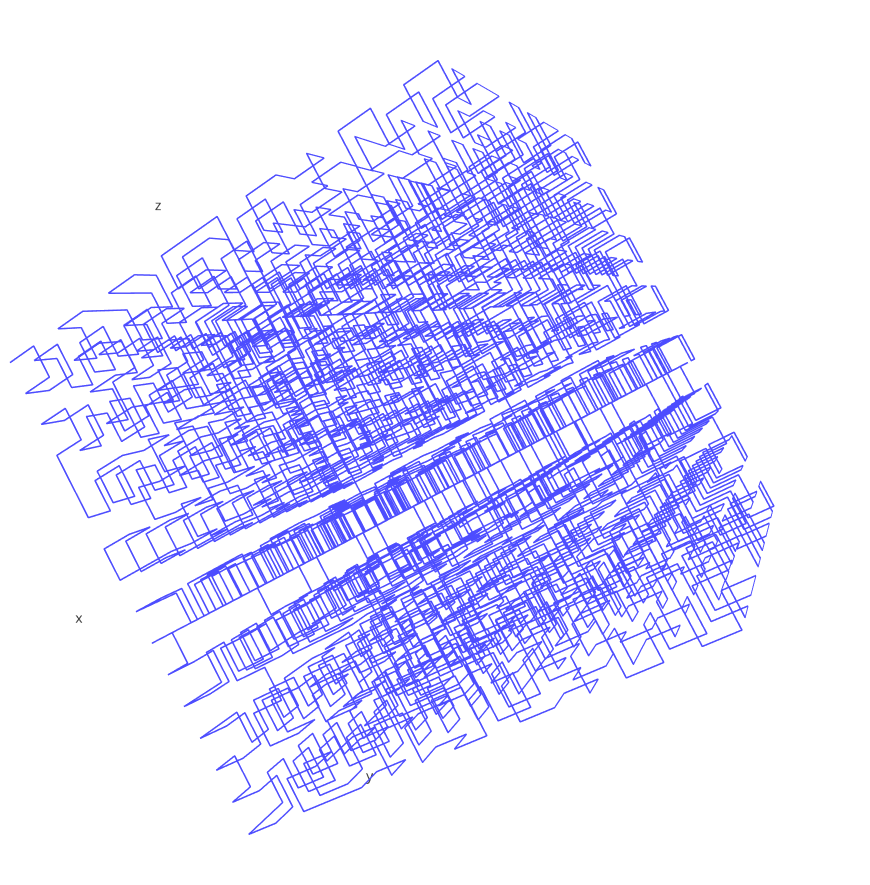
\includegraphics[width=.3\textwidth]{peano3d.png}
    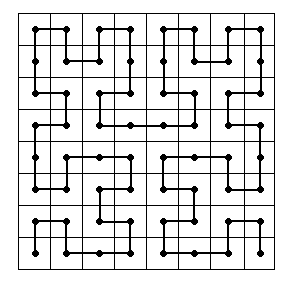
\includegraphics[width=.3\textwidth]{peano2d.png}
  \end{figure}
\end{center}
\end{frame}

\begin{frame}
  \frametitle{Свойства задачи после редукции}
  После применения развёртки, \(\varphi(y(x))\) удовлетворяет условию Гёльдера:
  \begin{displaymath}
    |\varphi(y(x_1))-\varphi(y(x_2))|\leq H{|x_1-x_2|}^{\frac{1}{N}}, x_1,x_2\in[0,1],
  \end{displaymath}
  \(\varphi(y(x))\) является негладкой функцией с множеством локальных и глобальных экстремумов \textbf{global}, даже если \(\varphi(y)\) унимодальна.
  Появление дополнительных экстремумов связано с потерей информации о \(N\)-мерной окрестностях точек после преобразования в одномерное пространство.

  \begin{figure}[ht]
    \begin{center}

    \vspace*{-0.5cm}
    \subfloat{\raisebox{.02\textheight}{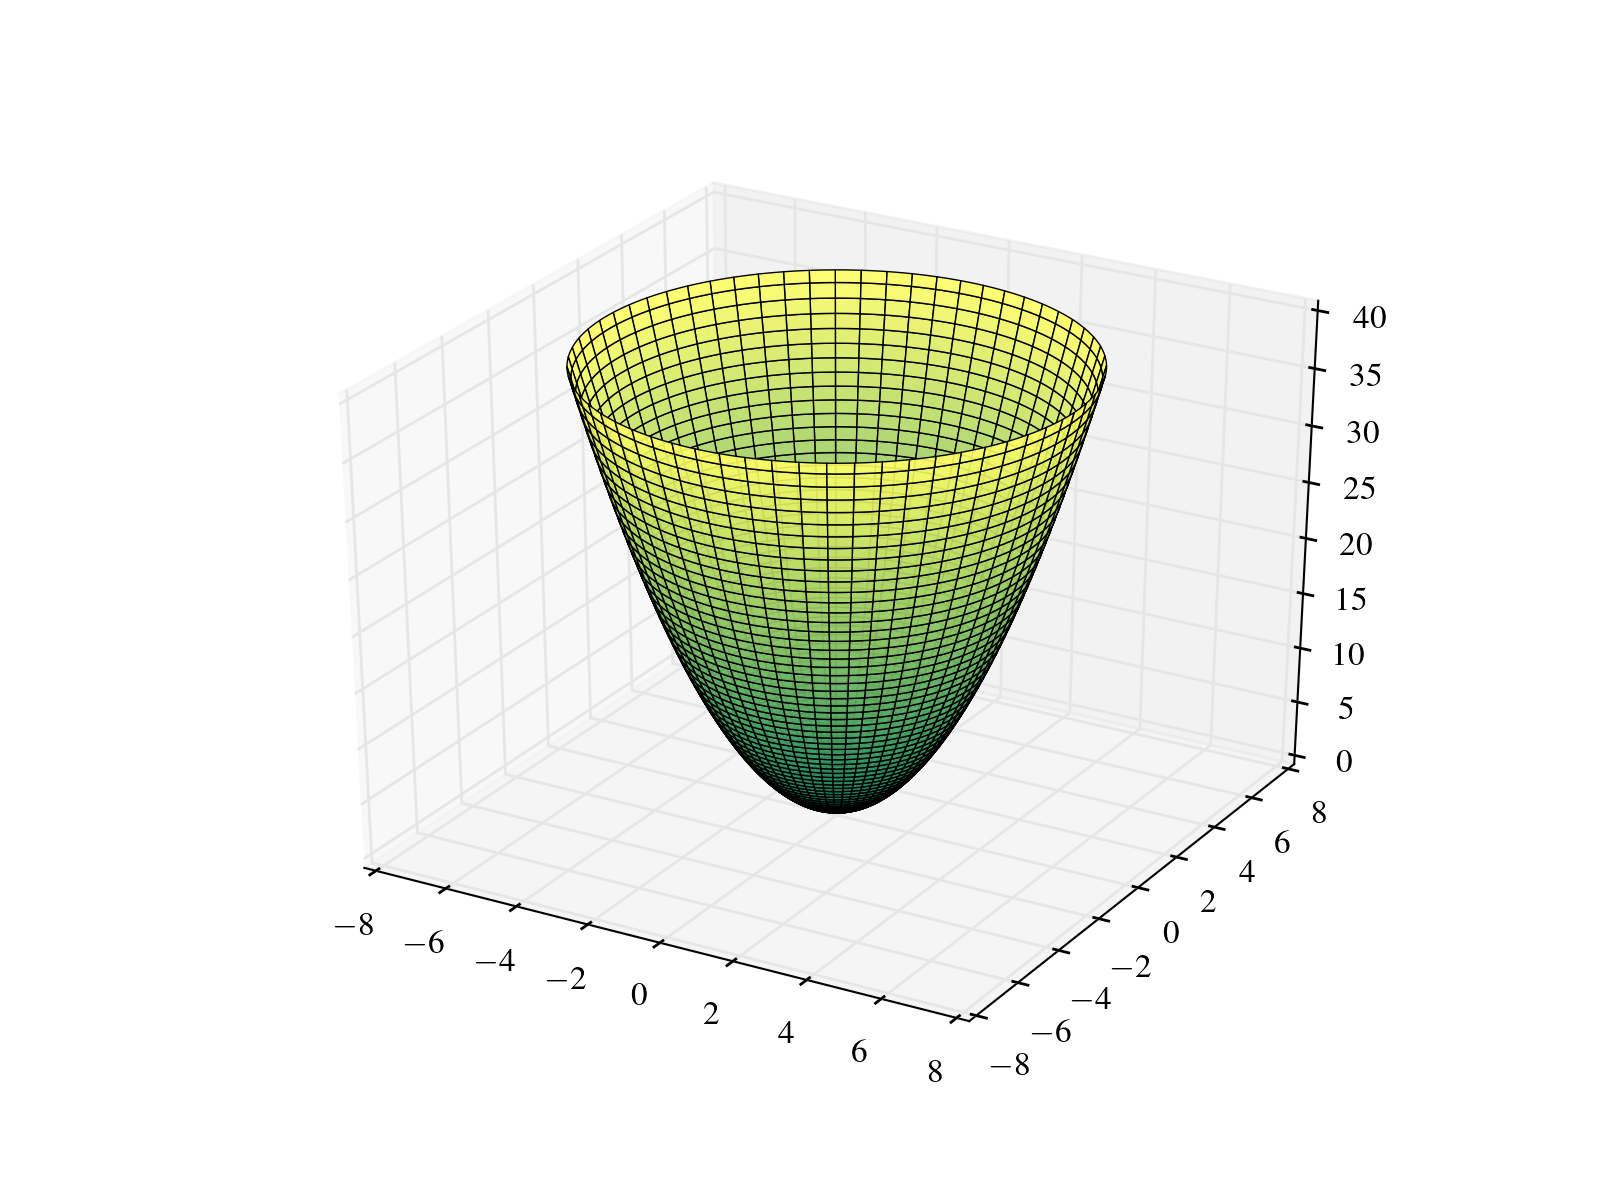
\includegraphics[width=.3\textwidth]{parabaloid.png}}}
    \subfloat{\raisebox{.2\textheight}{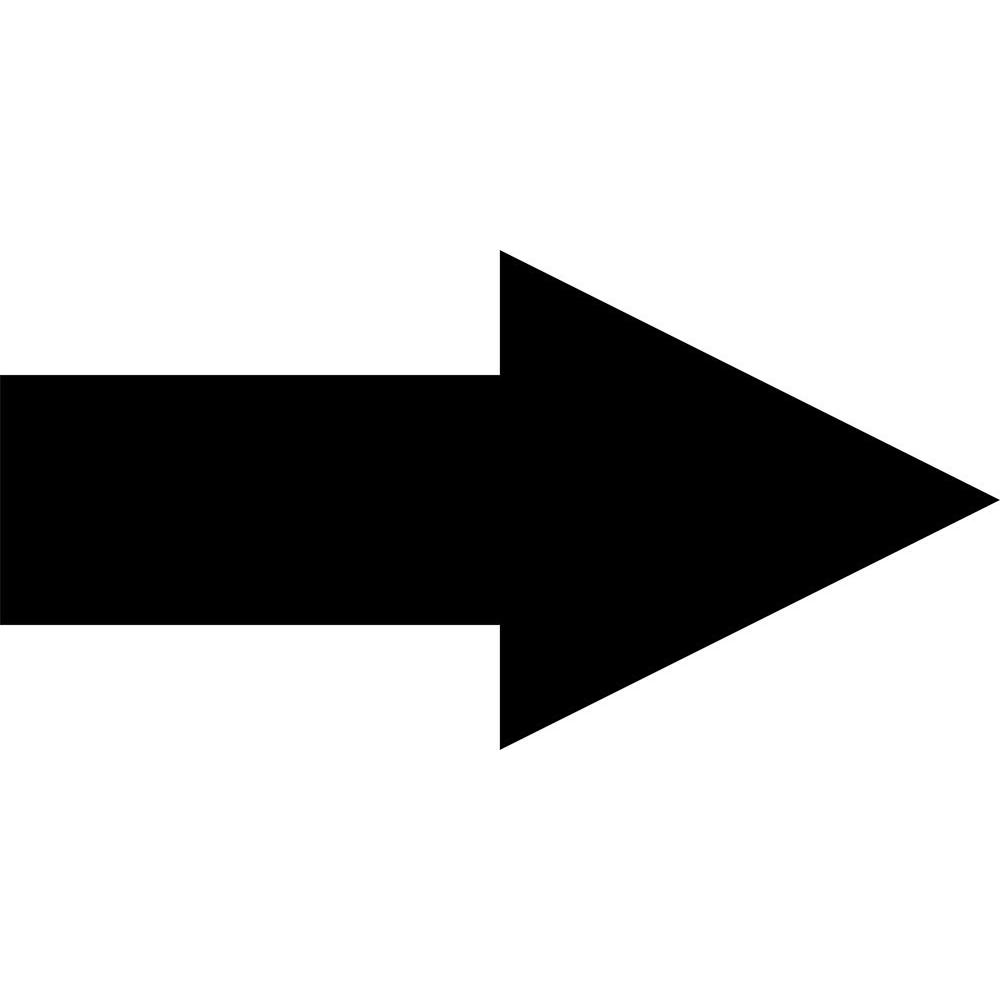
\includegraphics[width=.05\textwidth]{arrow.jpg}}}
    \subfloat{{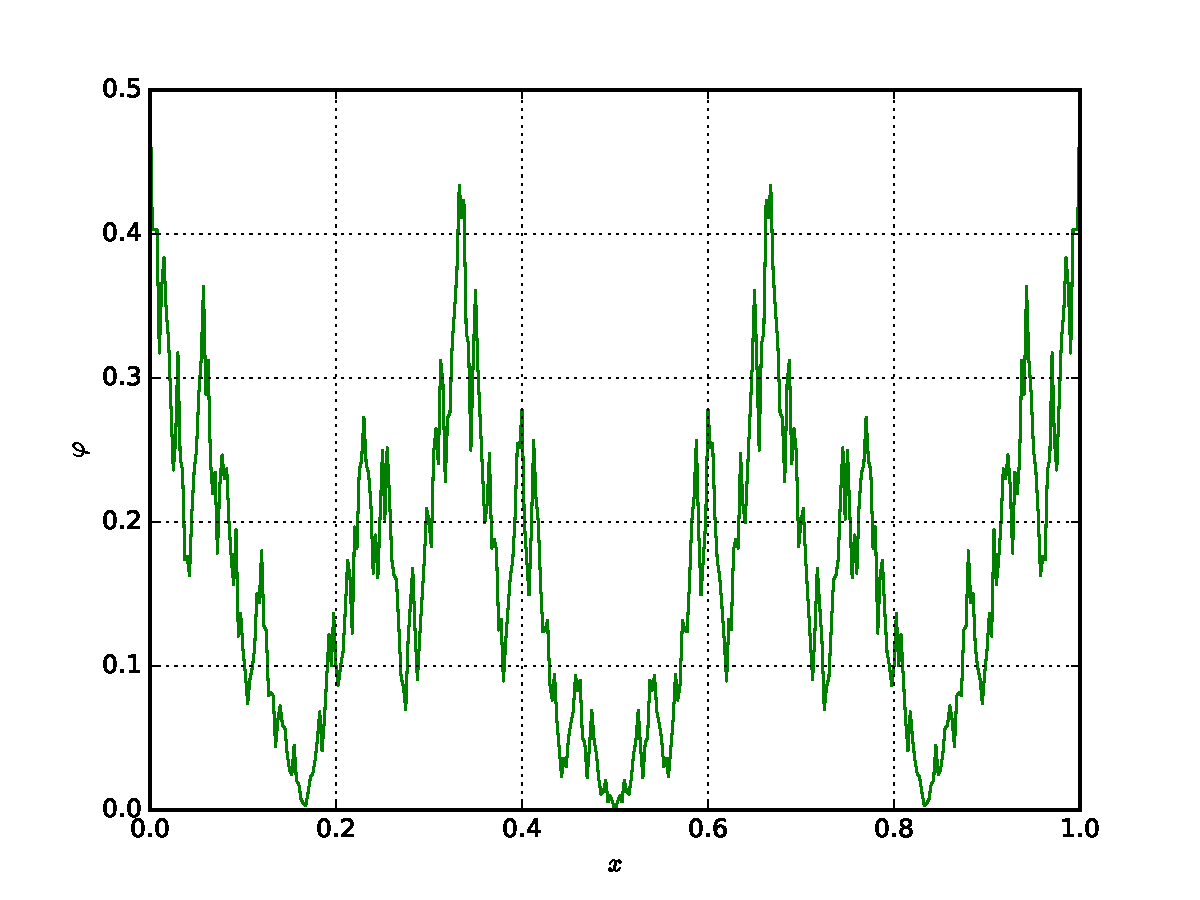
\includegraphics[width=.45\textwidth]{map_paraboloid.pdf}}}
  \end{center}
  \end{figure}
\end{frame}

\begin{frame}
  \frametitle{Одномерный алгоритм глобального поиска (AGS)}
  Optimization method generates search sequence \(\{x_k:x_k\in[a,b]\}\) and consists of the following steps:
  \begin{enumerate}
    \setlength{\itemindent}{.1in}
    \item[Step 1.] Sort the search information (one-dimensional points) in increasing order.
    \item[Step 2.] For each interval \((x_{i-1}, x_i)\) compute quantity \(R(i)\), called characteristic.
    \item[Step 3.] Choose an interval with the greatest characteristic, \((x_{t-1}, x_{t})\), and
    make a trial (compute the constraints and objective) at the point \(x^{k+1}\), chosen according with decision rule \(d\):
    \begin{displaymath}
      x^{k+1}=d(t)\in (x_{t-1}, x_{t})
    \end{displaymath}
    \item[Step 4.] If \(x_{t}-x_{t-1}<\varepsilon\) stop the method.
  \end{enumerate}
  \textit{\footnotesize	{Детальное описание приведено в Strongin R.G., Sergeyev Ya.D.: Global optimization with non-convex constraints. Sequential and parallel algorithms (2000), Chapter 7}}
\end{frame}

\begin{frame}
  \frametitle{Non-univalent evolvent}
    One can try to recover all preimages of \(y\in\mathbb{R}^N\) and make optimization method aware of their existence\footnote{R.G. Strongin. Numerical Methods in Multiextremal Problems (in Russian), 1978}. This allows reducing the effect of growing amount of local minimas after dimension reduction.
    According to the theory of Peano-type curves, each \(N\)-d point could have up to \(2^N\) preimages. For large \(N\) such preimages mining would be expensive.
      \begin{figure}[ht]
        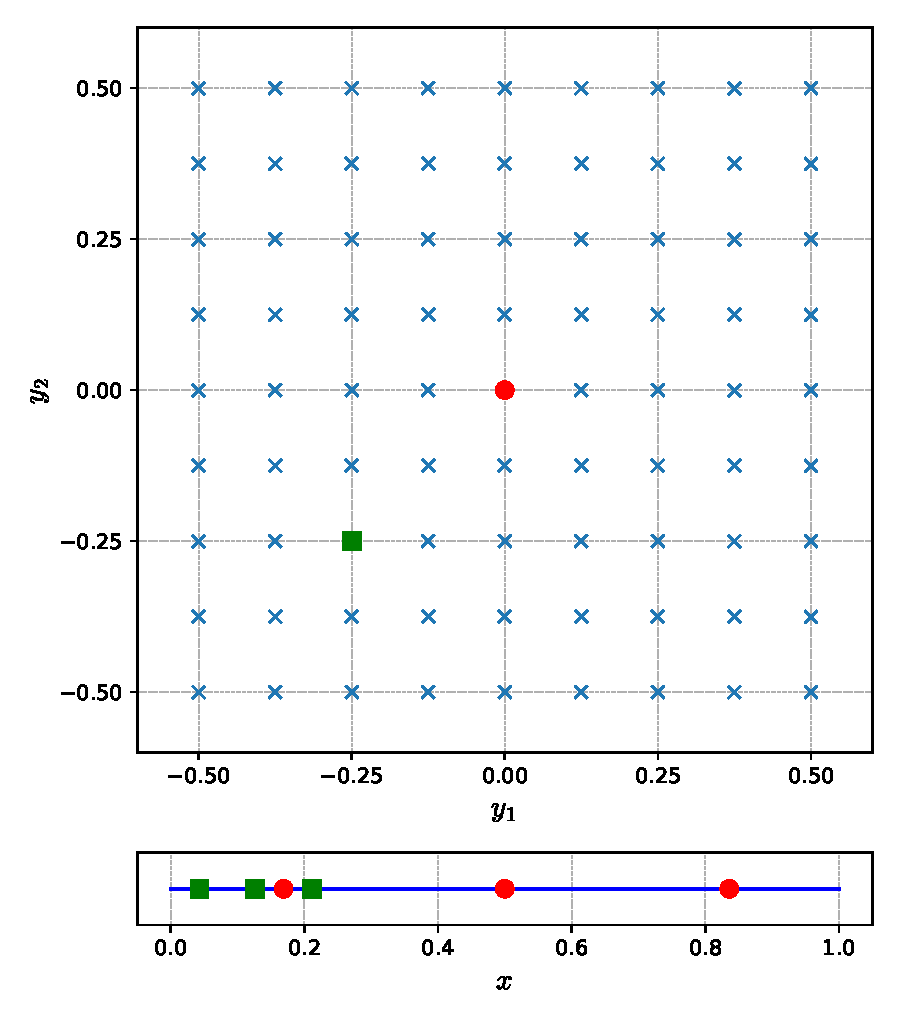
\includegraphics[width=.25\textwidth]{evolvents/noninjective.pdf}
      \end{figure}
\end{frame}

\begin{frame}
  \frametitle{Shifted and rotated evolvents}
  To create a fixed amount of preimages one can use a pre-defined set of different evolvents. These evolvents could be shifted or rotated versions of the original one. Set of shifted evolvents\footnote{Strongin, R.G. Algorithms for multi-extremal mathematical programming problems employing the set of joint space-filling curves, Journal of Global Optimization 2(4), 357--378, 1992} is theoretically proven to generate at least one pair of close preimages if their images are close and it performs better than the a set of rotated curves in that sense.
  \begin{figure}[ht]
    \subfloat{\raisebox{.0\textheight}{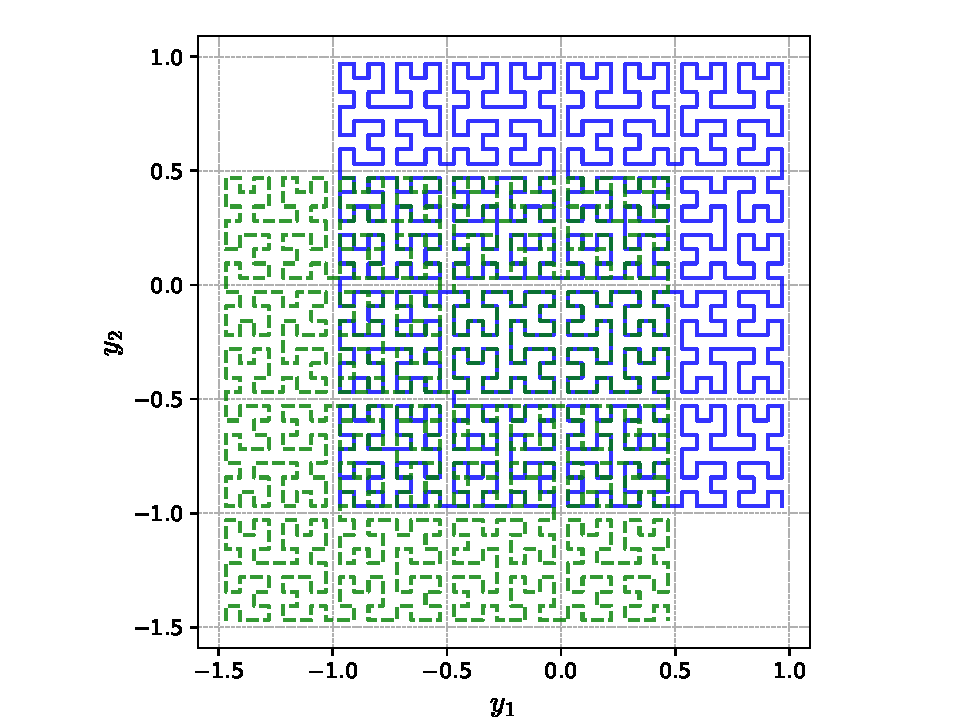
\includegraphics[width=.35\textwidth]{evolvents/shifted.pdf} }}
    \subfloat{{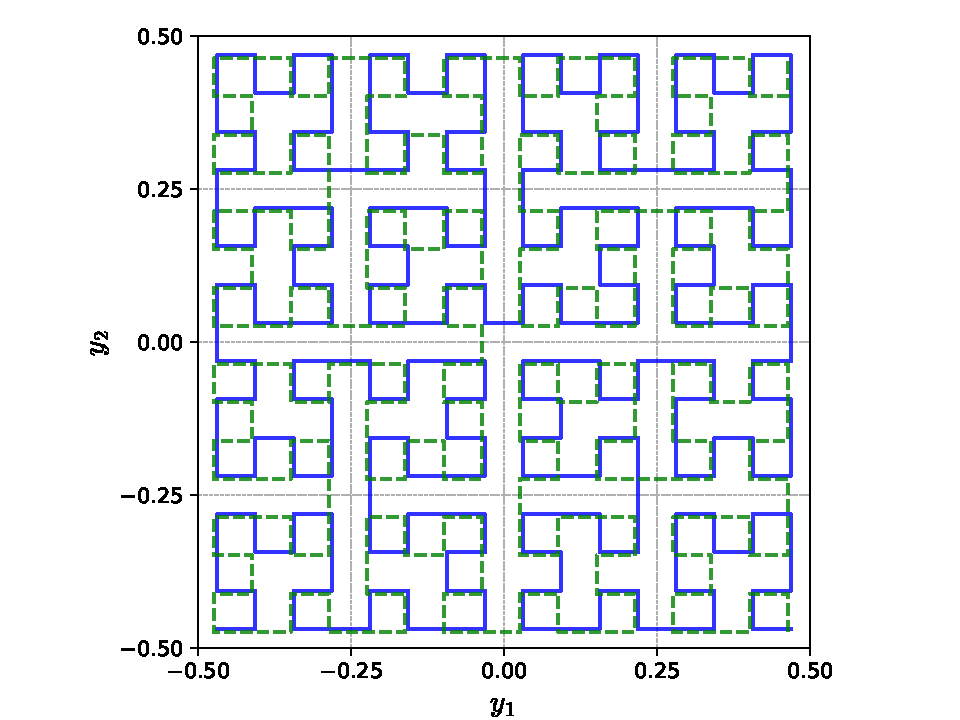
\includegraphics[width=.35\textwidth]{evolvents/rotated.pdf} }}
  \end{figure}
\end{frame}

\begin{frame}
  \frametitle{Smooth evolvent}
  Smooth functions are more predictable for optimizer, so smooth approximation of the Peano-like \(y(x)\) curve could improve convergence rate \footnote{Goryachih, A. A class of smooth modification of space-filling curves for global optimization problems, NET 2016}.
  \begin{figure}[ht]
    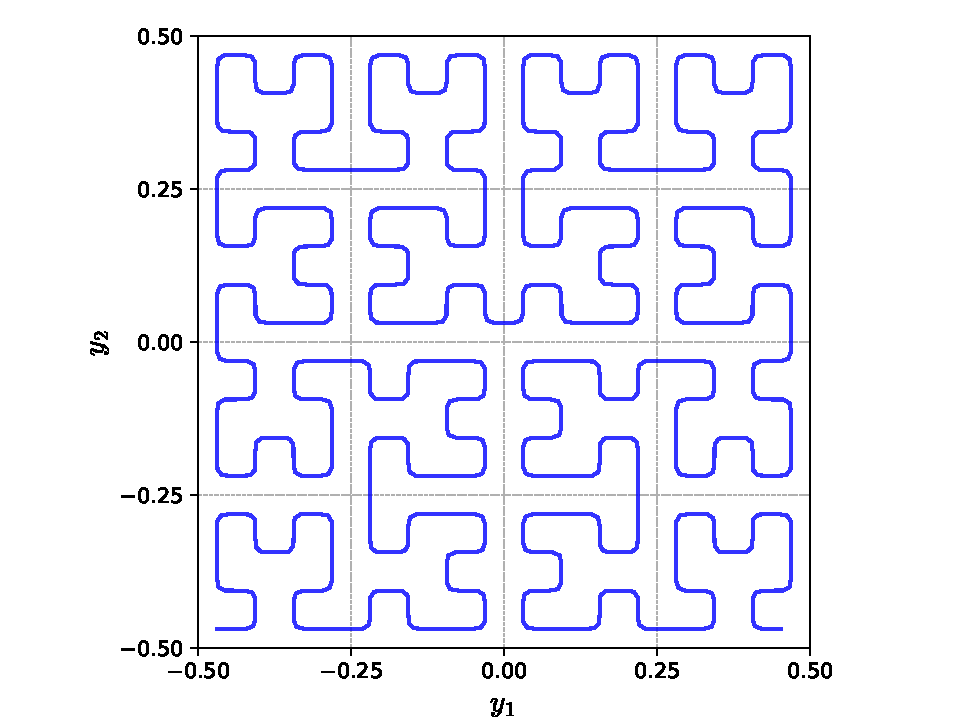
\includegraphics[width=0.45\textwidth]{evolvents/smooth.pdf}
  \end{figure}

\end{frame}

\begin{frame}
  \frametitle{Evolvents comparison}
  \begin{figure}[ht]
    \hspace*{-0.9cm}
    \subfloat[Minimal \(r\)]{{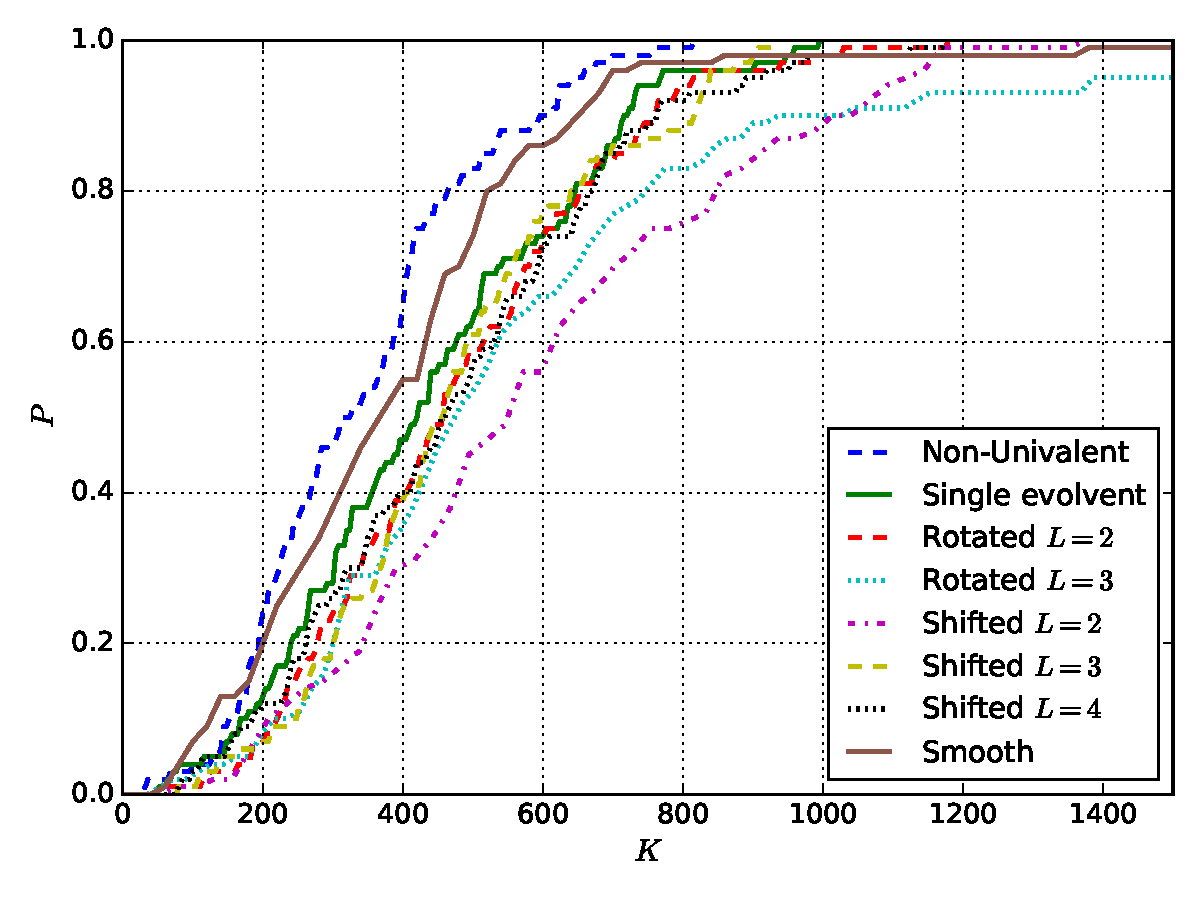
\includegraphics[width=.55\textwidth]{evolvents/gklsS2d_opt_pt_op.pdf} }}
    \subfloat[\(r=5.0\)]{{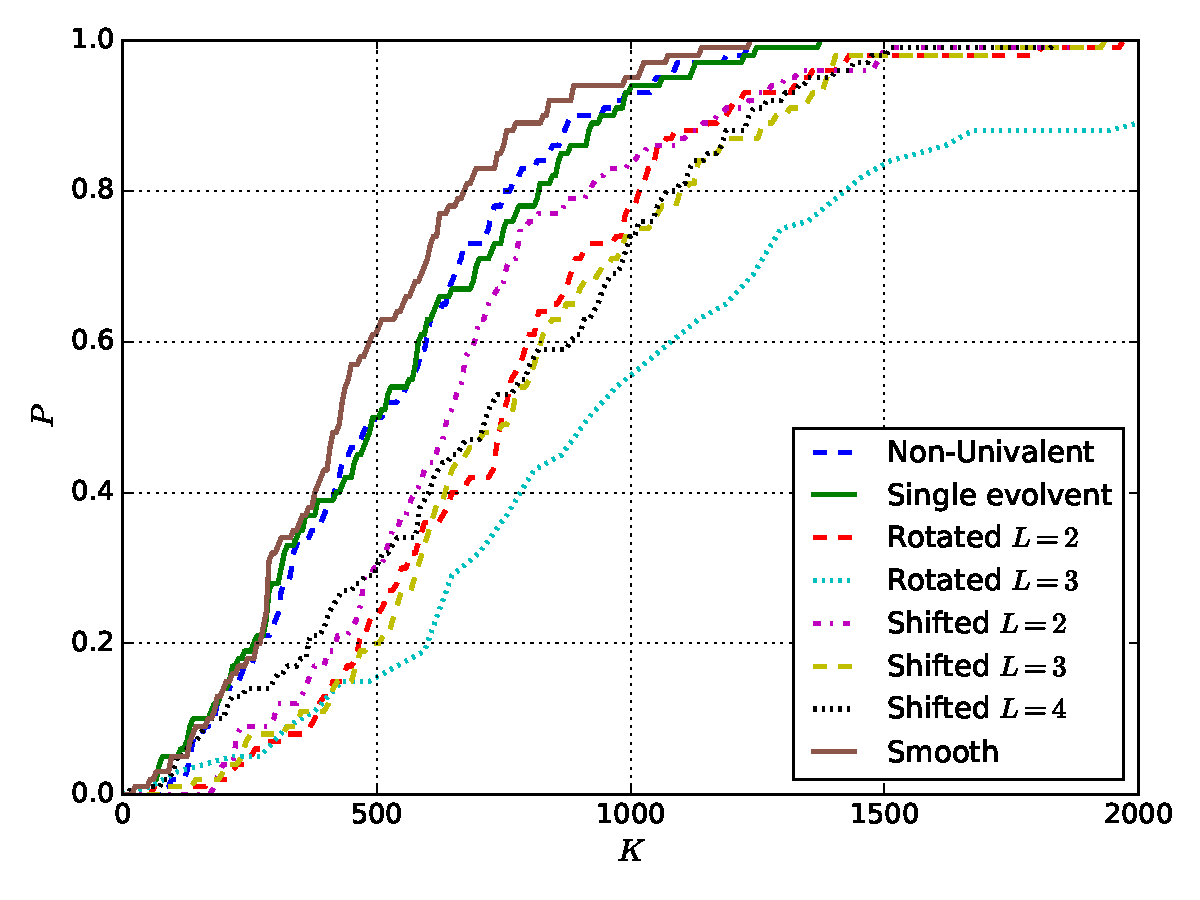
\includegraphics[width=.55\textwidth]{evolvents/gklsS2d_same_r_opt_pt_op.pdf} }} \hspace*{4cm}
    \caption{Operating characteristics on GKLS 2d Simple class}
  \end{figure}
\end{frame}

\begin{frame}
  \frametitle{Evolvents comparison}
  \begin{figure}[ht]
    \hspace*{-0.9cm}
    \subfloat[Minimal \(r\)]{{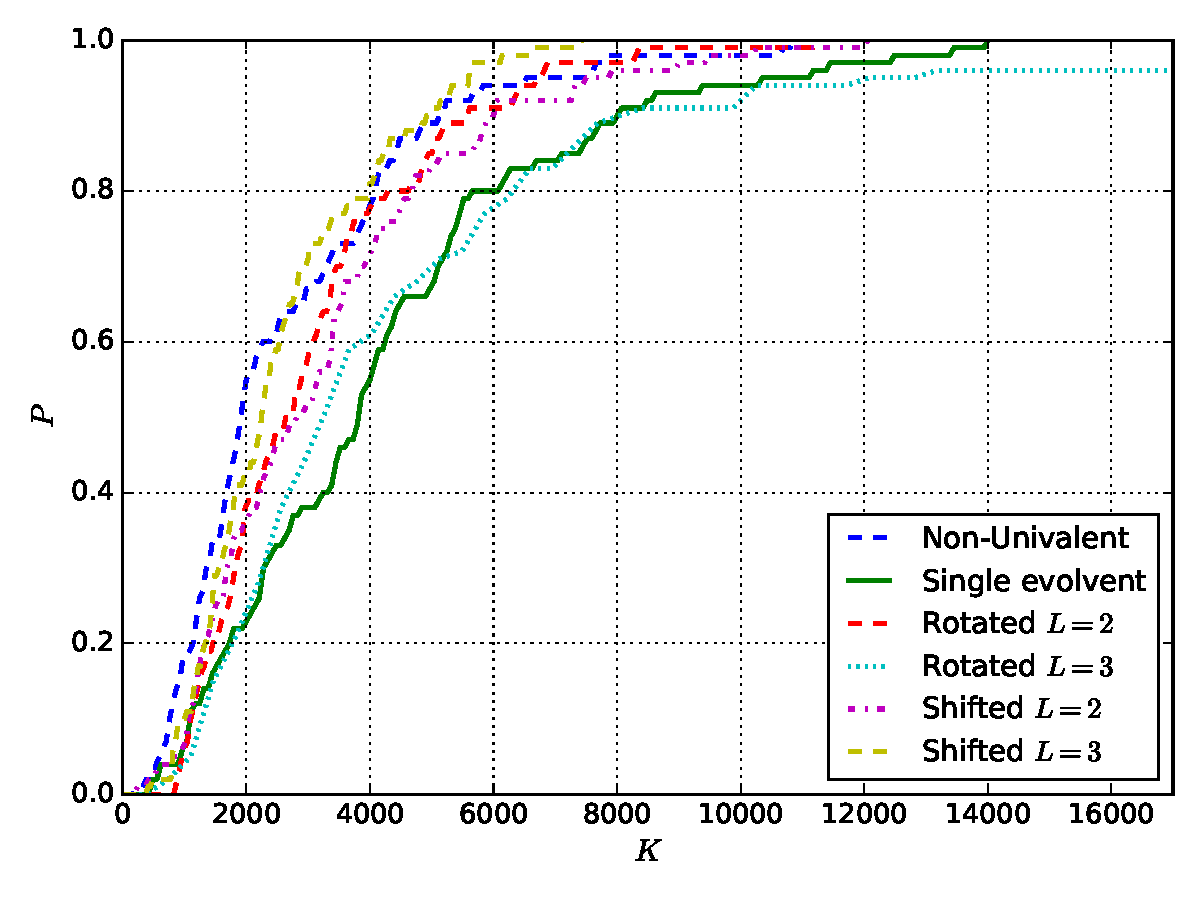
\includegraphics[width=.55\textwidth]{evolvents/gklsS3d_opt_pt_op.pdf} }}
    \subfloat[\(r=4.5\)]{{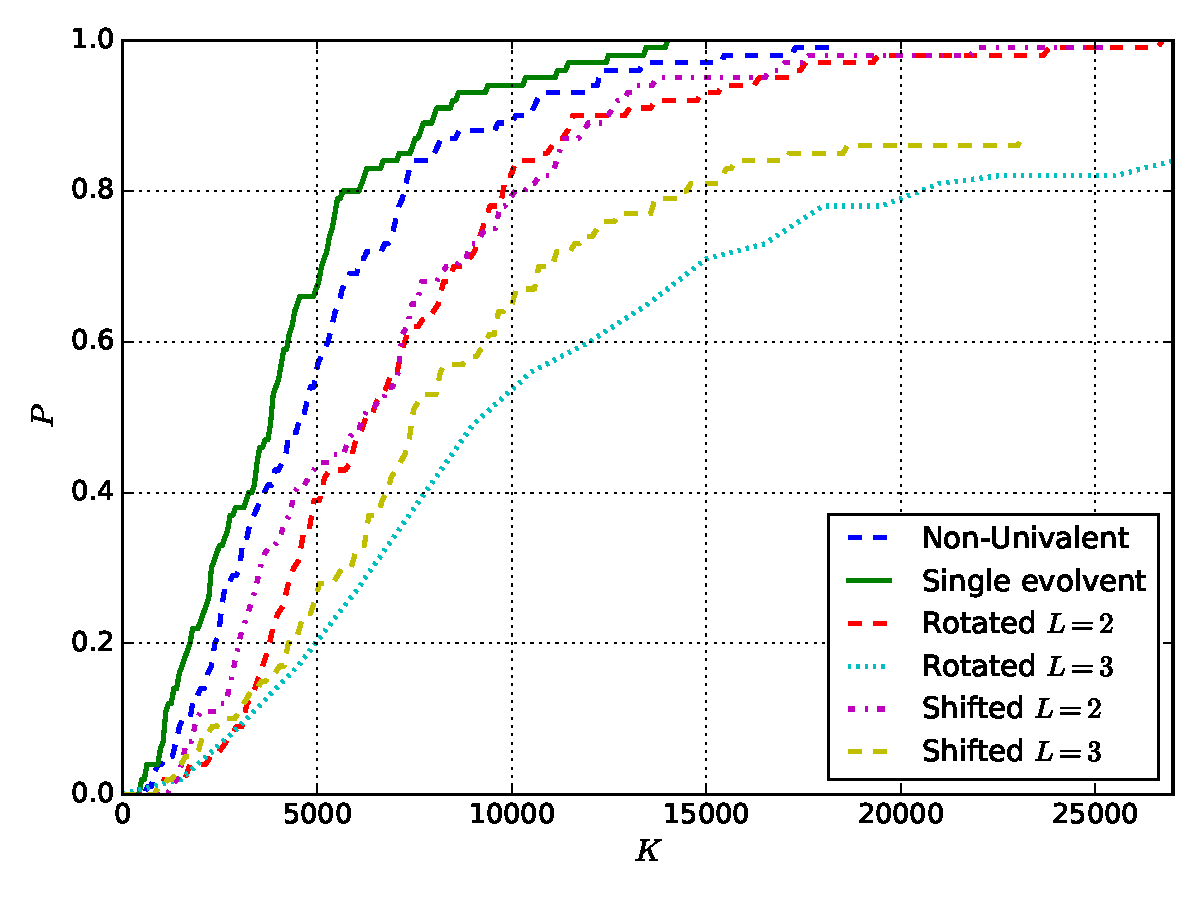
\includegraphics[width=.55\textwidth]{evolvents/gklsS3d_same_r_opt_pt_op.pdf} }}
    \caption{Operating characteristics on GKLS 3d Simple class}
  \end{figure}
\end{frame}


\begin{frame}
  \frametitle{Methods}
  In this work considered the following solvers available in open-source:
  \begin{itemize}
    \item[$\square$] \textbf{Deteriminstic}:
    \begin{itemize}
      \item DIRECT, DIRECT$l$ (Gablonsky J. M. et al, 2001);
      \item AGS (Strongin R.G., 1978).
    \end{itemize}
    \item[$\square$] \textbf{Stochastic}:
    \begin{itemize}
      \item Multi Level Single Linkage (Alexander H. G. et al, 1987);
      \item StoGO (Madsen, Kaj at al, 1998);
      \item Differential Evolution (Storn, Rainer et al, 1997);
      \item Controlled Random Search (Price, W. L., 1983);
      \item Dual Simulated Annealing (Y Xiang et al, 1997);
    \end{itemize}
  \end{itemize}
\end{frame}

\begin{frame}
  \frametitle{Hyperparameters tuning in AGS}
  In order to resolve the problem of choosing $r$ to some extent,
  let us use the following scheme:
  \begin{itemize}
    \item execute $q$ iterations of AGS with $r=r_{max}$;
    \item execute $q$ iterations of AGS with $r=r_{min}$;
    \item repeat the above steps either until convergence or until the allowed number of iterations are
  exhausted.
\end{itemize}
  Now we have 3 parameters instead of one, but the method is not so sensitive to them.
  Let $q=50\cdot\log_2(N-1)\cdot N^2$, $r_{min}=3,\:r_{max}=2\cdot r_{min}$ in all the future experiments.
\end{frame}


\begin{frame}
  \frametitle{Results of different methods}
  \begin{figure}[ht]
    \centering
    \subfloat[4d Simple]{{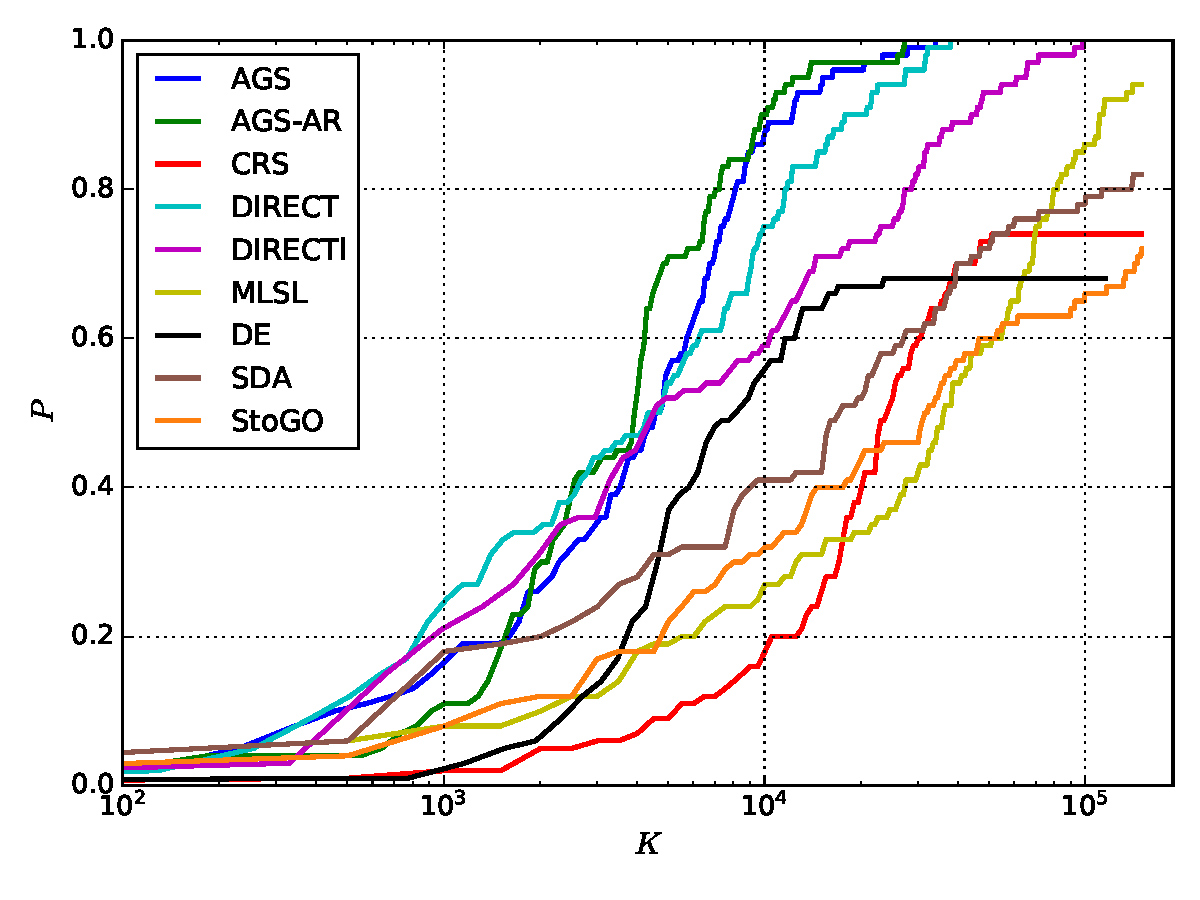
\includegraphics[width=.5\textwidth]{comparison/gklss4d.pdf}}\label{fig:s4d}}
    \subfloat[4d Hard]{{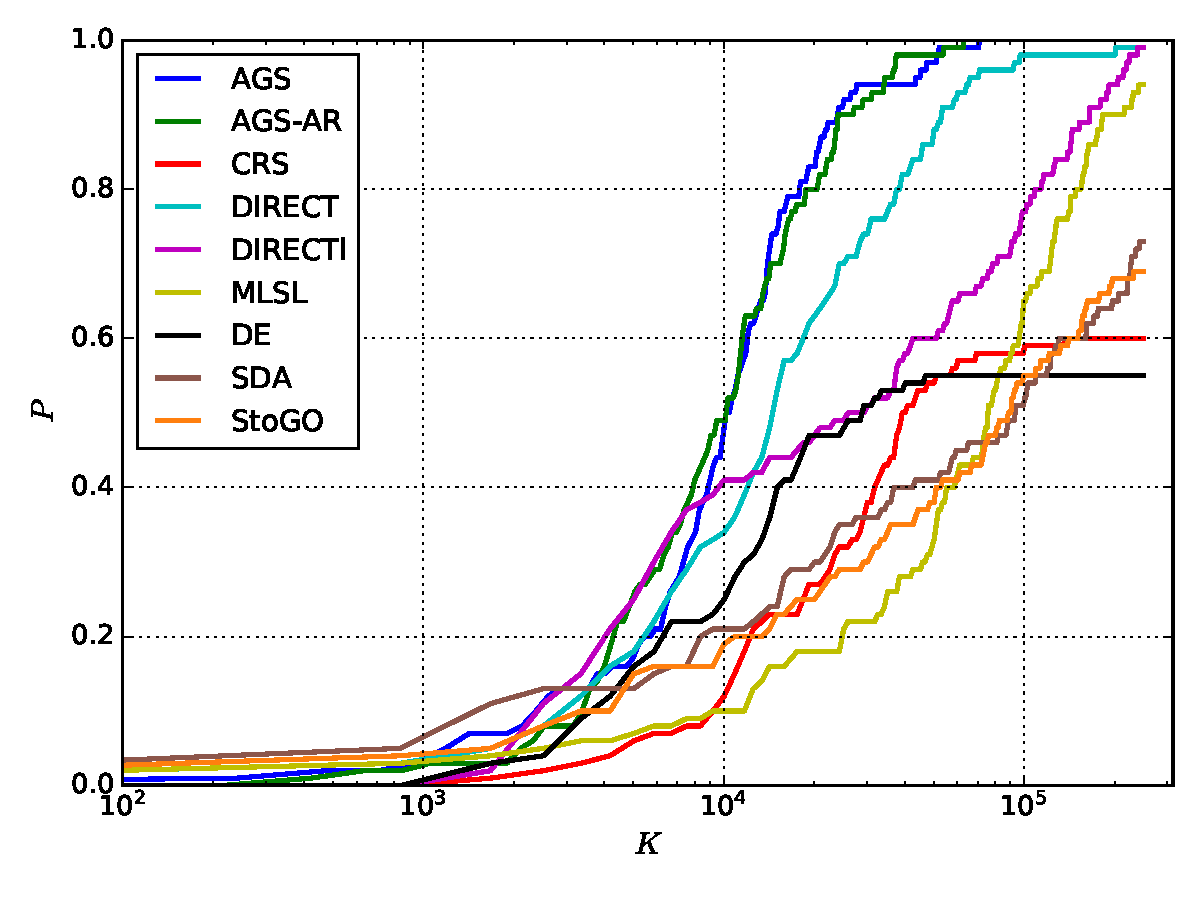
\includegraphics[width=.5\textwidth]{comparison/gklsh4d.pdf}}\label{fig:h4d}}
  \end{figure}
\end{frame}

\begin{frame}
  \frametitle{Results of different methods}
  \begin{figure}[ht]
    \centering
    \subfloat[5d Simple]{{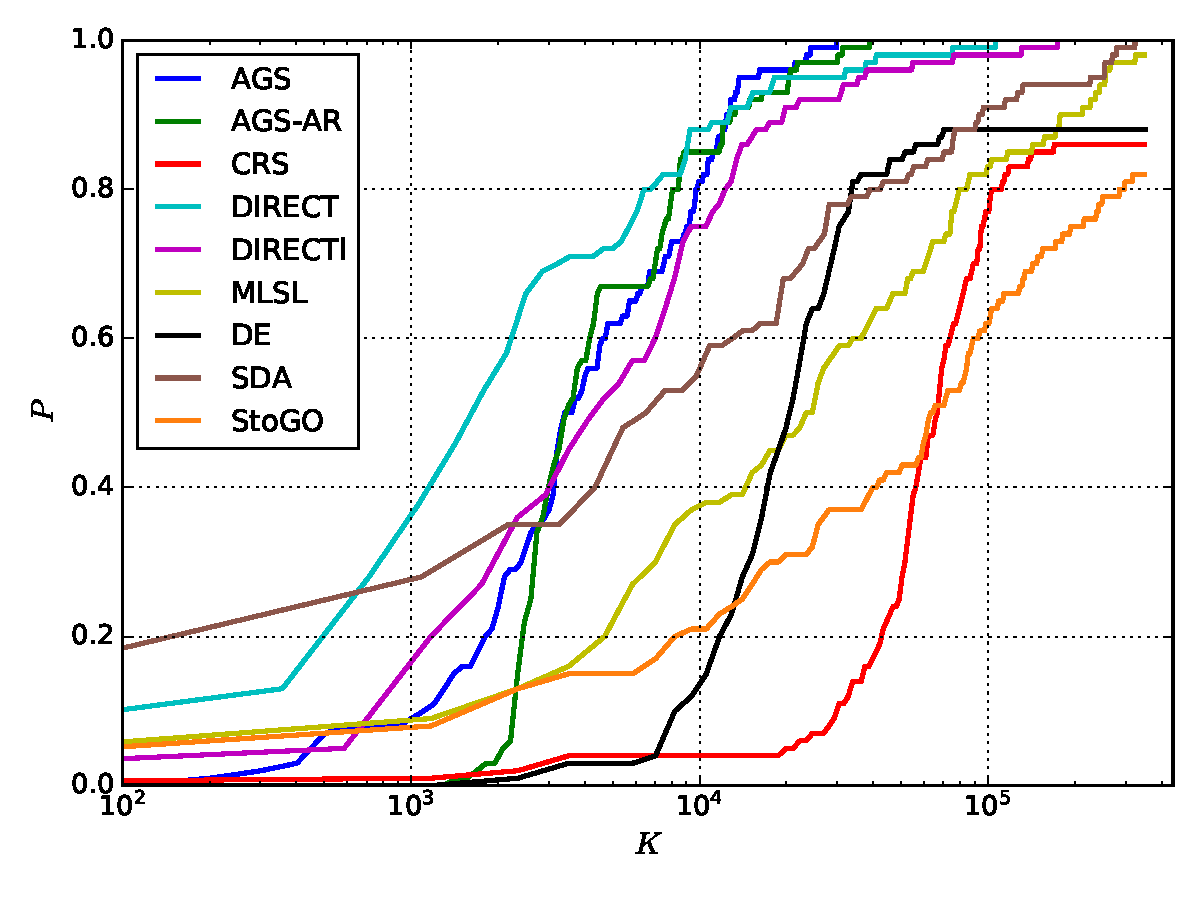
\includegraphics[width=.5\textwidth]{comparison/gklss5d.pdf}}\label{fig:s4d}}
    \subfloat[5d Hard]{{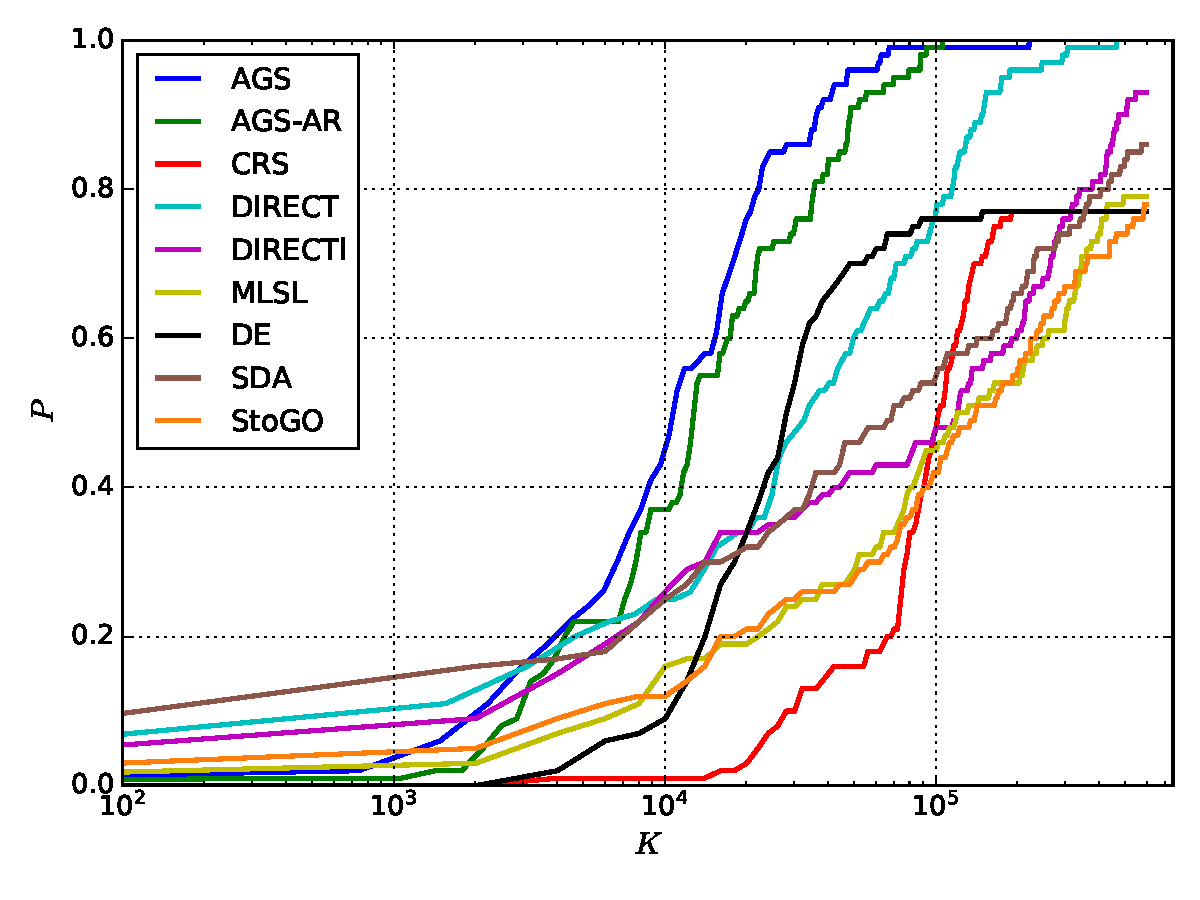
\includegraphics[width=.5\textwidth]{comparison/gklsh5d.pdf}}\label{fig:h4d}}
  \end{figure}
\end{frame}


\begin{frame}
  \frametitle{Algorithm for solving a set of problems}
  The method relies on the previously introduced AGS and consists of the following steps:
  \begin{itemize}
    \item Create \(q\) copies of AGS.
    \item Run \(q\) synchronously working copies of AGS, but instead of performing Step 3, stop all
    the methods and select an interval with the highest characteristic among intervals from all the methods.
    \item If the interval with the highest characteristic belongs to problem \(i\), execute Step 3 in the \(i^{th}\) copy of AGS.
    Other copies skip Step 3.
    \item To implement parallel processing, method picks \(p\) intervals at the previous two steps
    and performs \(p\) trials simultaneously.
  \end{itemize}
  The described method relies to \textbf{comparability of characteristics in different problems}.
\end{frame}

\begin{frame}
  \frametitle{Index method of handling inequality constraints}
  Instead of the original problems with functional constraints the index scheme considers the following unconstrained problem:
  \begin{displaymath}
    \begin{array}{lr}
      \psi (x^{*})=\min_{x\in [0;1]}\psi (x), \\
      \psi (x)={\begin{cases}g_{\nu }(x)/H_{\nu }&\nu <M\\(g_{M}(x)-g_{M}^{*})/H_{M}&\nu =M\end{cases}},
    \end{array}
  \end{displaymath}
  where if \(\nu=m+1\;,g_\nu(x)=\varphi(x)\).

  Characteristics are defined as follows:
  \begin{displaymath}
    R(i)={\begin{cases}\Delta _{i}+{\frac {(z_{i}-z_{i-1})^{2}}{(r_{\nu }\mu _{\nu })^{2}\Delta _{i}}}-2{\frac {z_{i}+z_{i-1}-2z_{\nu }^{*}}{r_{\nu }\mu _{\nu }}}&\nu =\nu (x_{i})=\nu (x_{i-1})\\2\Delta _{i}-4{\frac {z_{i-1}-z_{\nu }^{*}}{r_{\nu }\mu _{\nu }}}&\nu =\nu (x_{i-1})>\nu (x_{i})\\2\Delta _{i}-4{\frac {z_{i}-z_{\nu }^{*}}{r_{\nu }\mu _{\nu }}}&\nu =\nu (x_{i})>\nu (x_{i-1})\end{cases}}
  \end{displaymath}
  where \(z_i=\psi(x_i)\).
\end{frame}

\begin{frame}
  \frametitle{Univariate Algorithm of Global Search}
  Sufficient convergence conditions:
  \begin{enumerate}
    \item \(G\ne\emptyset\), the source problem has a solution.
    \item Functions \(g_j(y)\leqslant 0, 1\leqslant j\leqslant m + 1\), are Lipschitzian with
respective constants \(L_i\) over the domain \(D\) (here \(g_{m+1}(y)=\varphi(y)\)).
    \item During the optimization process estimations of \(L_i\) becomes large enough.
  \end{enumerate}
\end{frame}

\begin{frame}
  \frametitle{An example of solving a multi-objective problem}
  Consider the following problem:
  \begin{displaymath}
    \begin{array}{l}
        Minimize \left \{
        \begin{array}{l}
          f_1(y) = 4 y_1^2 + 4 y_2^2 \\
          f_2(y) = (y_1-5)^2 + (y_2-5)^2 \\
        \end{array}
        \right .
        y_1\in [-1;2],y_2\in [-2;1]
        \\s.t.
        \\
        \left \{
        \begin{array}{l}
          g_1(y) = (y_1 - 5)^2 + y_2^2 - 25 \leqslant 0 \\
          g_2(y) = -(y_1 - 8)^2 - (y_2 + 3)^2 + 7.7 \leqslant 0\\
        \end{array}
        \right .
    \end{array}
  \end{displaymath}
  After scalarization the problem has the following form:
  \begin{displaymath}
    \varphi(y^*(\lambda_1,\lambda_2))=\min_{y\in D}\max\{\lambda_1 f_1(y), \lambda_2 f_2(y)\};\lambda_1,\lambda_2\in[0,1],\: \lambda_1+\lambda_2=1
\end{displaymath}
To build the Pareto set numerically, consider
100 pairs of the variables \((\lambda_1,\lambda_2)\) such that
\(\lambda_1^i=i h,\: \lambda_2^i=1-\lambda_1^i,\: h=10^{-2},i=\overline{1, 100}\).
\end{frame}

\begin{frame}
  \frametitle{An example of solving a multi-objective problem}
  \vspace*{-1.0cm}
  \begin{displaymath}
    \begin{array}{cr}\\
      SP(S)=\sqrt{\frac{1}{|S|-1} \sum_{i=1}^{|S|} (\overline{d}-d_i)^2},\:\overline{d}=mean\{d_i\}, \\
      d_i=\min_{s_i,s_j\in S:s_i\ne s_j}||F(s_i)-F(s_j)||_1,\: F=(f_1,f_2)
    \end{array}
  \end{displaymath}

  \begin{figure}[ht]
      \centering
      \vspace*{-0.5cm}
      \subfloat[IAGS, \(SP_{single}=0.984\)]{
      \label{fig:mco_pareto_1} {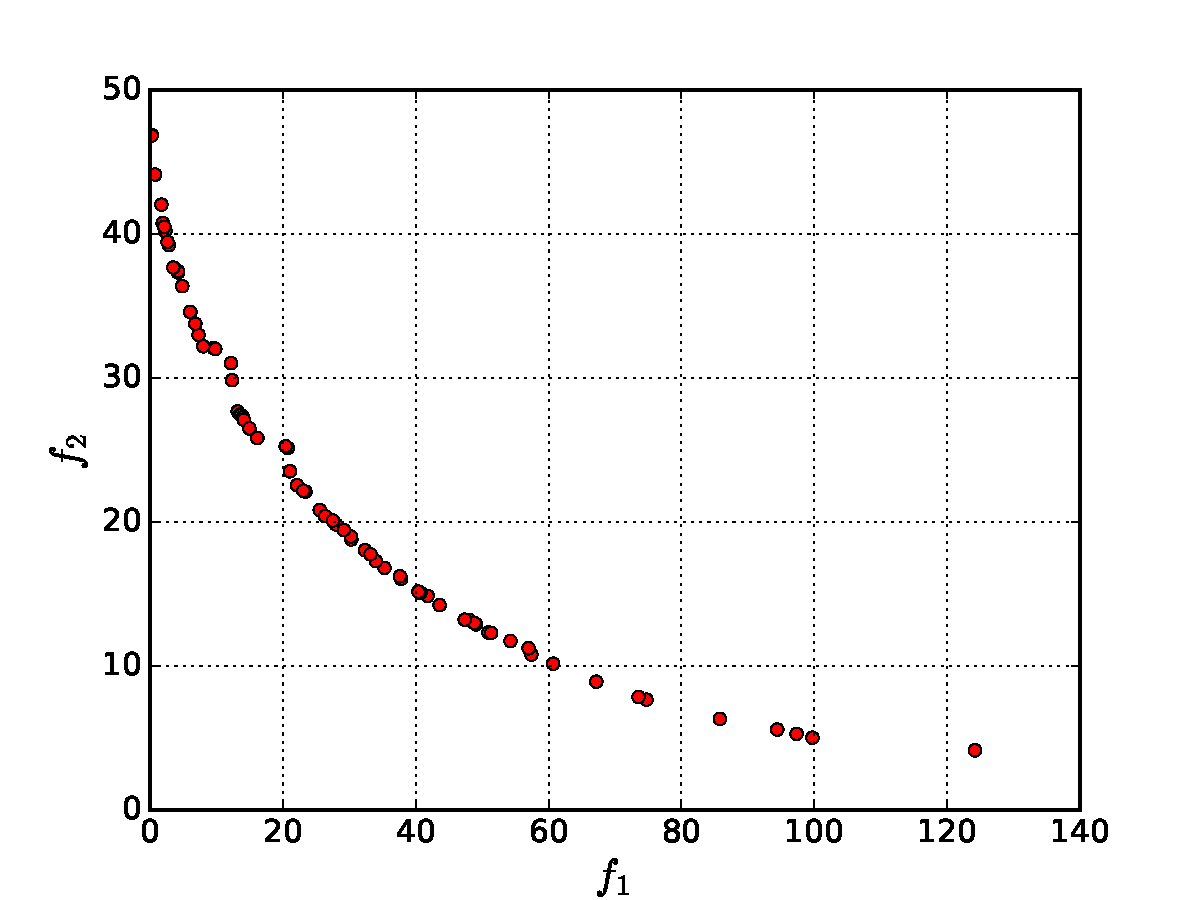
\includegraphics[width=.5\textwidth]{single_mco.pdf}}}
      \subfloat[MIAGS, \(SP_{multi}=0.749\)]{
      \label{fig:mco_pareto_2} {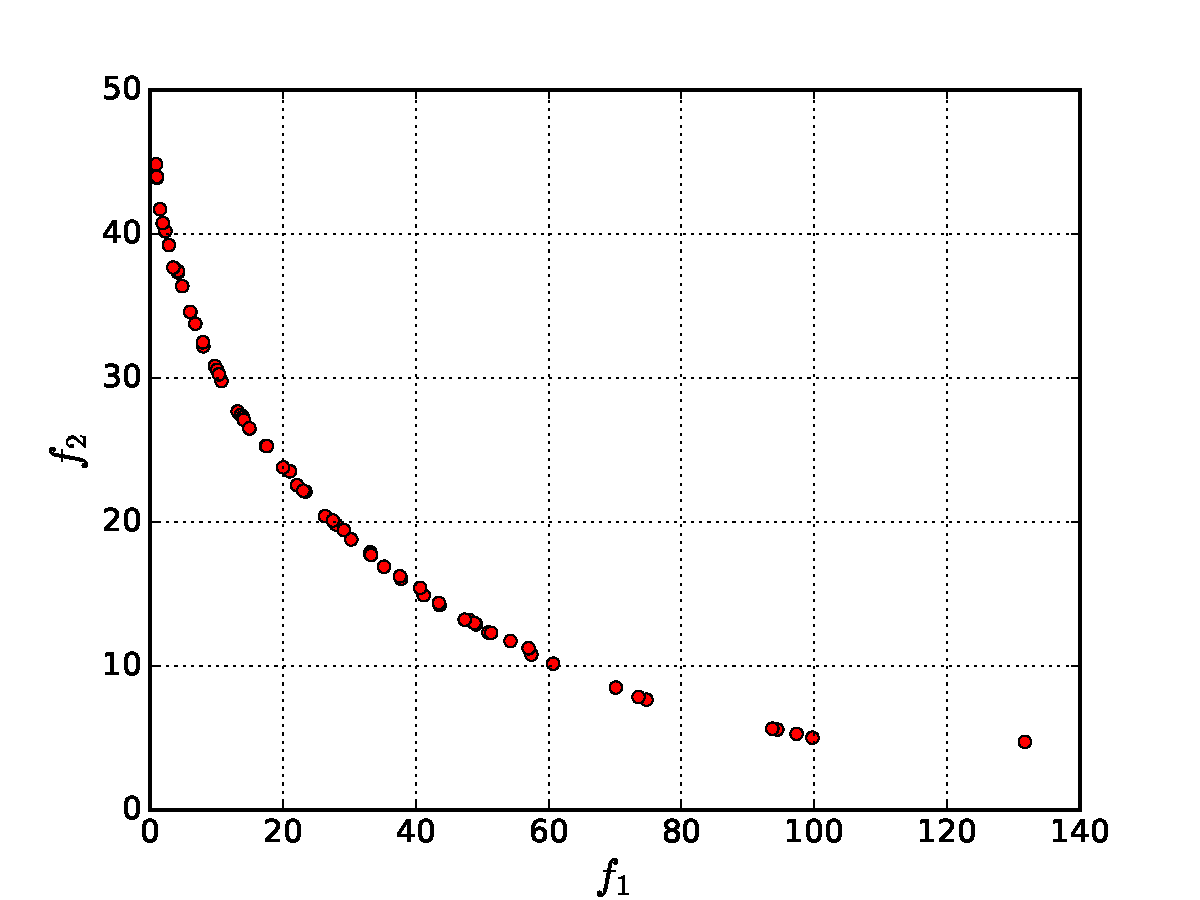
\includegraphics[width=.5\textwidth]{multi_mco.pdf}}}
      \caption{Numerical estimations of the Pareto set, obtained after 2500 trails}
      \label{fig:mco_pareto}
  \end{figure}
\end{frame}

\begin{frame}
  \frametitle{Generated test problems}
  \begin{columns}
    \begin{column}{0.5\textwidth}
      Sets of test problems are obtained by applying the GCGen system to
      functions produced by generators of unconstrained test problems.
      The main features of the generated sets:
      \begin{itemize}
        \item \(q\)=100;
        \item Dimension 2, 3 or 4;
        \item Base fuctions GKLS or \(F_{GR}\), or a combination of them;
        \item Number of nonlinear constraints: 2.
      \end{itemize}
    \end{column}
    \begin{column}{0.5\textwidth}
      \centerline{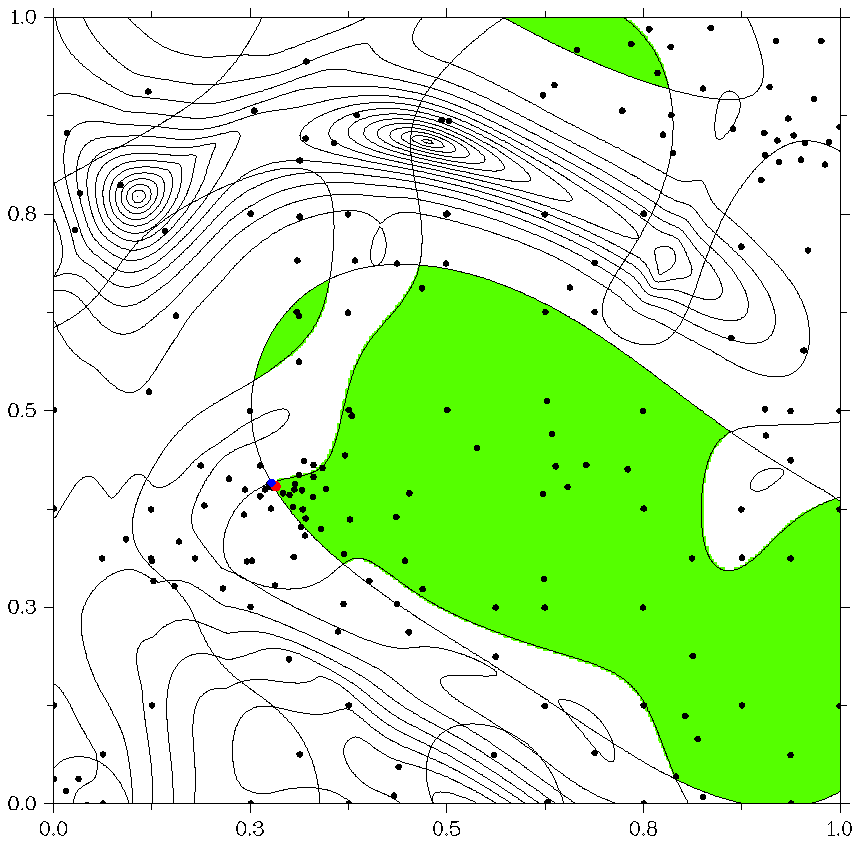
\includegraphics[width=0.9\textwidth]{4.png}}
    \end{column}
  \end{columns}
  \footnotesize{GCGen is available here: \textit{https://github.com/UNN-ITMM-Software/GCGen}}
\end{frame}

\begin{frame}
  \frametitle{Hardware and software environment}
  \begin{center}
    The parallel method was implemented on C++ language with the use of OpenMP
    technology for organizing parallelism on shared memory.

    All the numerical experiments were carried out on a computer with the following
    configuration: Intel Core i7-7800X (6 cores) CPU, 64GB RAM, Unubtu 16.04 ОS, GCC 5.5 compiler.
  \end{center}
\end{frame}

\begin{frame}
  \frametitle{Result of solving sets of synthetic problems}
  \begin{figure}[ht]
    \vspace*{-0.5cm}
      \centering
      \subfloat[\(D_{max}\)]{
      \label{fig:max_dev} {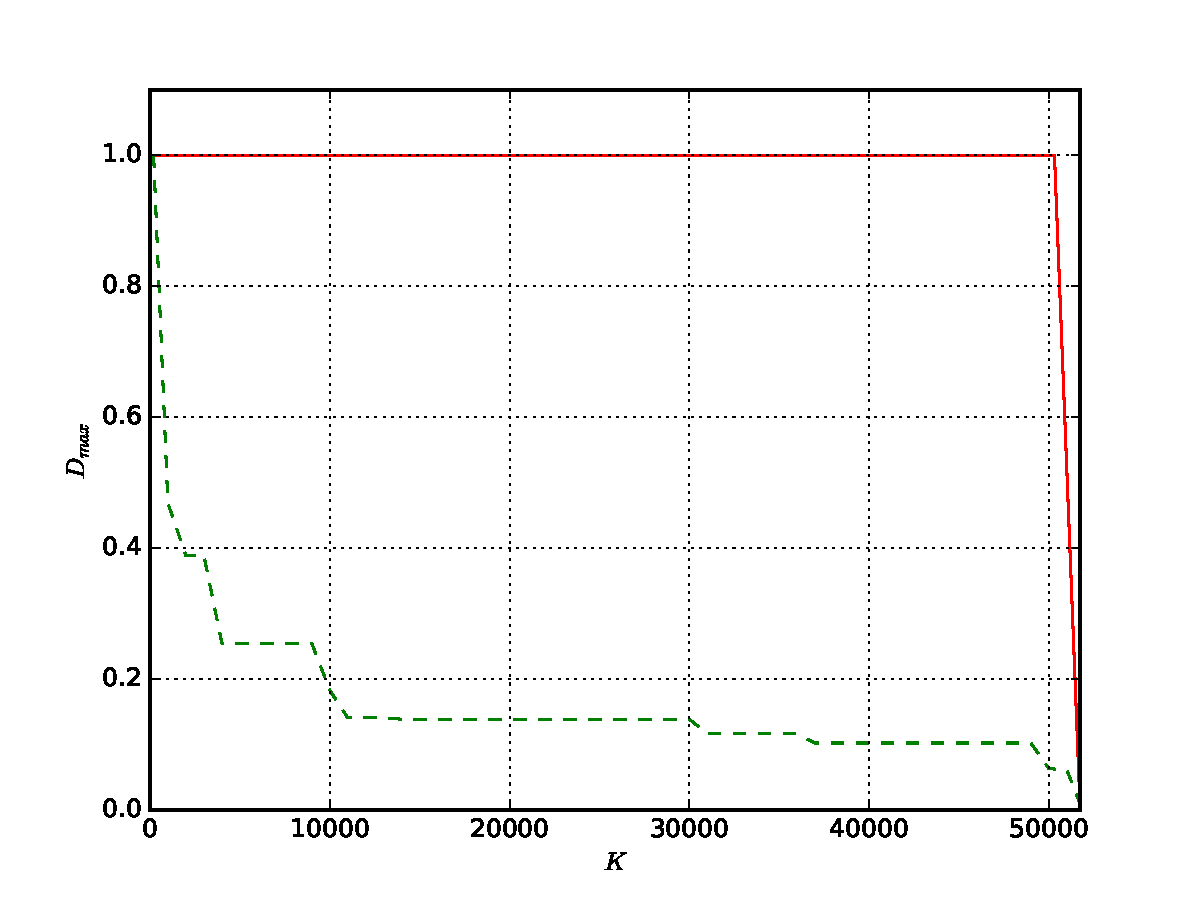
\includegraphics[width=.5\textwidth]{mixed_2d_max.pdf}}}
      \subfloat[\(D_{avg}\)]{
      \label{fig:avg_dev} {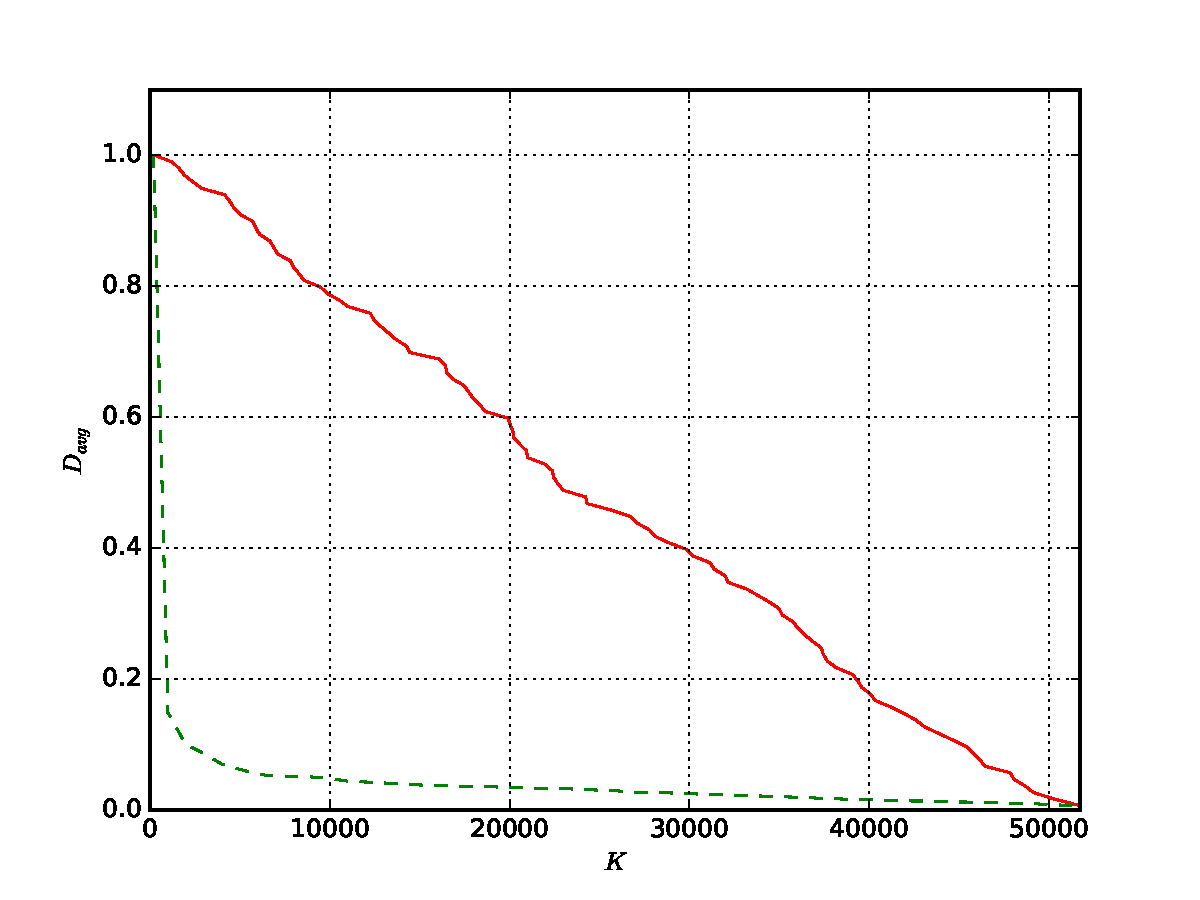
\includegraphics[width=.5\textwidth]{mixed_2d_avg.pdf}}}
      \caption{Dynamic of the average and maximal errors, during solving of problems
      generated on different types of base functions: GKLS и \(F_{GR}\)}
      \label{fig:devs_mixed}
  \end{figure}
\end{frame}

\begin{frame}
  \frametitle{Result of solving sets of synthetic problems}
  \begin{table}
    \centering
    \begin{tabular}{c|c|c|c|c|c}
      %\cline{1-8}\noalign{\smallskip}
      Problems class & \textit{p} & Number of iterations & Time, s & \(S_i\) & \(S_t\)   \\
      %s\noalign{\smallskip} \cline{4-5} \cline{7-8}  \noalign{\smallskip}
      \hline
      GKLS \& \(F_{GR}\)-based \
        & 1 & 51434 & 90.20 & -    & - \\
        & 2 & 25698 & 56.96 & 2.00 & 1.58 \\
        & 4 & 13015 & 36.67 & 3.95 & 2.46 \\
        & 6 & 8332  & 26.85 & 6.17 & 3.36 \\
      \hline
      GKLS-based 2d \
        & 1 & 59066 & 97.53 & -    & - \\
        & 2 & 29060 & 60.56 & 2.04 & 1.61 \\
        & 4 & 14266 & 38.92 & 4.14 & 2.51 \\
        & 6 & 9436  & 29.53 & 6.26 & 3.30 \\
      \hline
    \end{tabular}
  \end{table}
\end{frame}
\begin{frame}
  \frametitle{Result of solving sets of synthetic problems}
  \begin{table}
    \centering
    \begin{tabular}{c|c|c|c|c|c}
      %\cline{1-8}\noalign{\smallskip}
      Problems class & \textit{p} & Number of iterations & Time, s & \(S_i\) & \(S_t\)   \\
      %s\noalign{\smallskip} \cline{4-5} \cline{7-8}  \noalign{\smallskip}
      \hline
      GKLS-based 3d \
        & 1 & 782544 & 1117.55 & -    & - \\
        & 2 & 397565 & 752.92  & 1.97 & 1.48 \\
        & 4 & 208073 & 526.67  & 3.76 & 2.12 \\
        & 6 & 142089 & 445.45  & 5.50 & 2.51 \\
      \hline
      GKLS-based 4d \
        & 1 & 14021720 & 15806.6 & -    & - \\
        & 2 & 6313070 & 7254.85  & 2.22 & 2.18 \\
        & 4 & 3479344 & 4932.55  & 4.03 & 3.20 \\
        & 6 & 2783339 & 3955.38  & 5.04 & 3.99 \\
      \hline
    \end{tabular}
  \end{table}
\end{frame}
\begin{frame}
  \frametitle{Заключение}
  В ходе выполнения работы были получены следующие результаты:
  \begin{enumerate}
      \item Произведено сравнение различных способов редукции размерности, основанных на отображениях типа кривой Пеано;
      \item Предложена модификация AGS, AGS-AR, менее чувствительная к параметрам; AGS-AR продемонстрировал надёжность и скорость
      сходимости на уровне другого детерминированного метода, DIRECT,
      и превзошёл на рассмотренных тестовых задачах многие другие методы, реализации которых так же доступны в исходных кодах.
      Программная реализация метода AGS-AR прошла процедуру ревью и была включена в состав популярной библиотеки
      алгоритмов нелинейной оптимизации NLOpt;
      \item Реализована поддержка нелинейных ограничений в алгоритме, решающeм
      множество задач глобальной оптимизации в совокупности и распределяющего свои ресурсы так, чтобы
      обеспечивать равномерную сходимость во всех задачах. Доказано теорема о достаточных условиях сходимости
      полученного метода. Свойство равномерной сходимости проверено с помощью численного эксперимента.
  \end{enumerate}
\end{frame}

{
\unnumbered
\begin{frame}{{}}
  \frametitle{Q\&A}
  \begin{center}
    %\Large{Контакты:}
\vspace{0.5cm}

    sovrasov.vladislav@itmm.unn.ru

    https://github.com/sovrasov
  \end{center}
\end{frame}
}
\end{document}
